\section{Sentiment Analysis and Topic Modeling}~\label{sec:sentiments}
We sought to find out how the sentiments of news articles about AI have changed over time.
We first used \verb+nltk+ to extract sentiment intensity aggregates for each year.
We focused on four main sentiments: \emph{positive}, \emph{negative}, \emph{neutral}, and \emph{compound}.

\subsection{Overall Sentiment Shifts Over Time}~\label{subsec:sentiments-overall}

\begin{figure}[H]
  \centering
  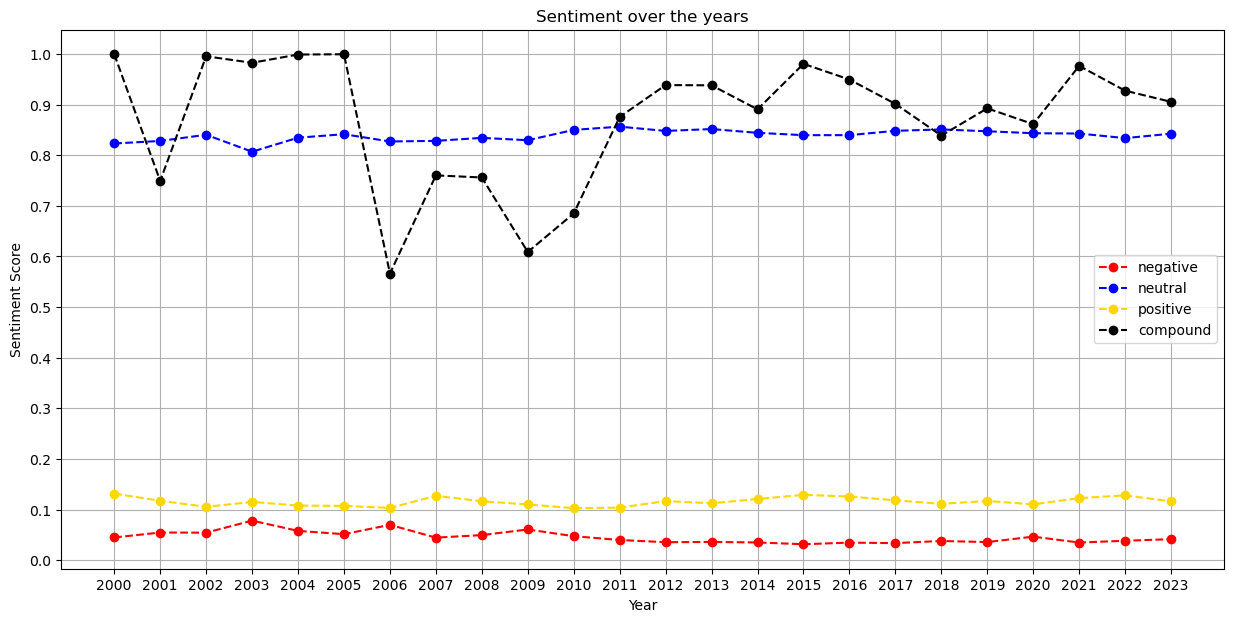
\includegraphics[width=\textwidth]{figures/sentiments/all.png}
  \caption{Sentiment analysis of articles about AI from $2000$ to $2023$.}
  \label{fig:sentiments}
\end{figure}

We notice little gradual changes in the \emph{positive}, \emph{negative}, and \emph{neutral} sentiments
over time. However, the \emph{compound} sentiment shows significant jumps and dips over time.

\subsection{Sentiment Shifts for the Top Ten Topics Over Time}~\label{subsec:sentiments-topics}

Since the composite sentiment score is a weighted average of other sentiment,
we are probably missing an important nuance in our data that is not captured by the three sentiments.

To try to understand this better, we used \emph{Latent Dirichlet Allocation} (LDA)
to extract the top-$10$ topics across the combined dataset then analyze how the sentiments
specific to each of those topics shift over time.

\newpage
\begin{figure}[H] % h! means put it here
  \centering
  \begin{subfigure}[b]{0.45\textwidth}
    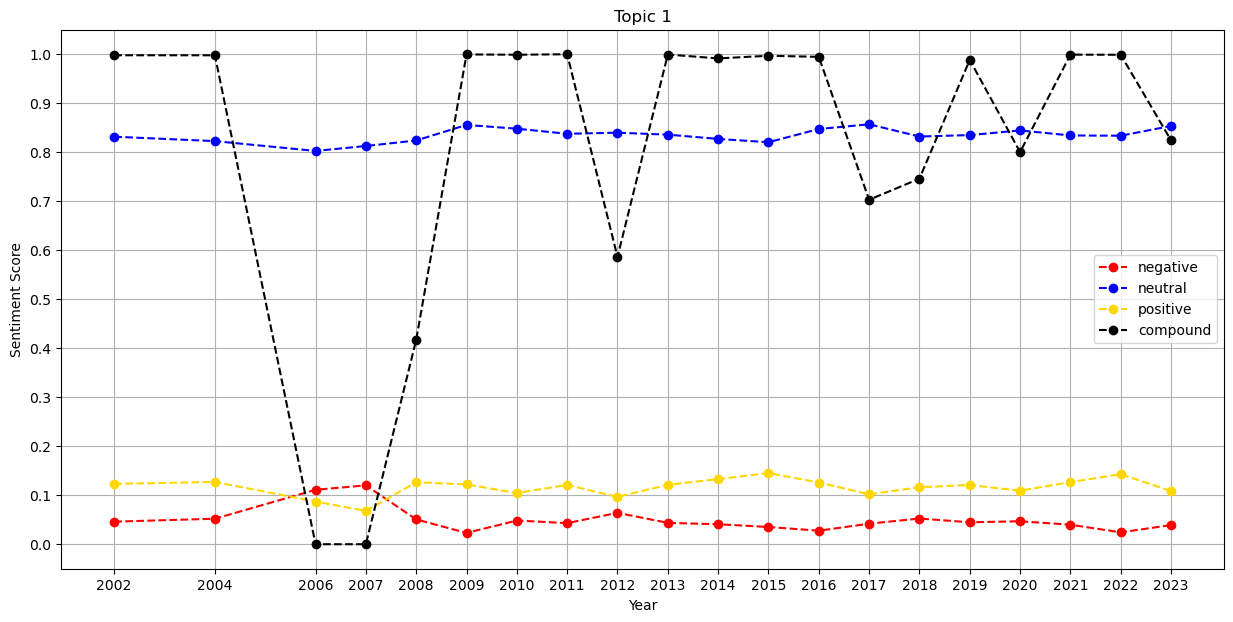
\includegraphics[width=\textwidth]{figures/sentiments/topic-1.png}
    \caption{\emph{chatbots, agents, twitter, privacy, ...}}
    \label{fig:sentiments-topic-1}
  \end{subfigure}
  \hfill
  \begin{subfigure}[b]{0.45\textwidth}
    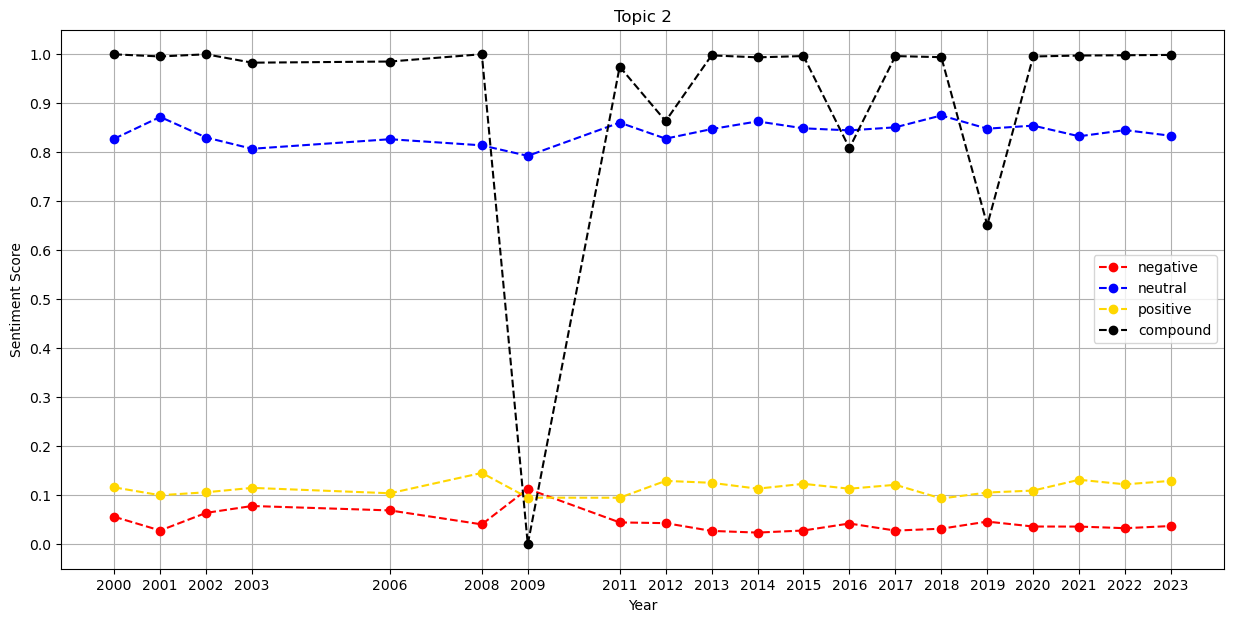
\includegraphics[width=\textwidth]{figures/sentiments/topic-2.png}
    \caption{\emph{google, data, intelligence, privacy, China...}}
    \label{fig:sentiments-topic-2}
  \end{subfigure}
  \vskip\baselineskip
  \begin{subfigure}[b]{0.45\textwidth}
    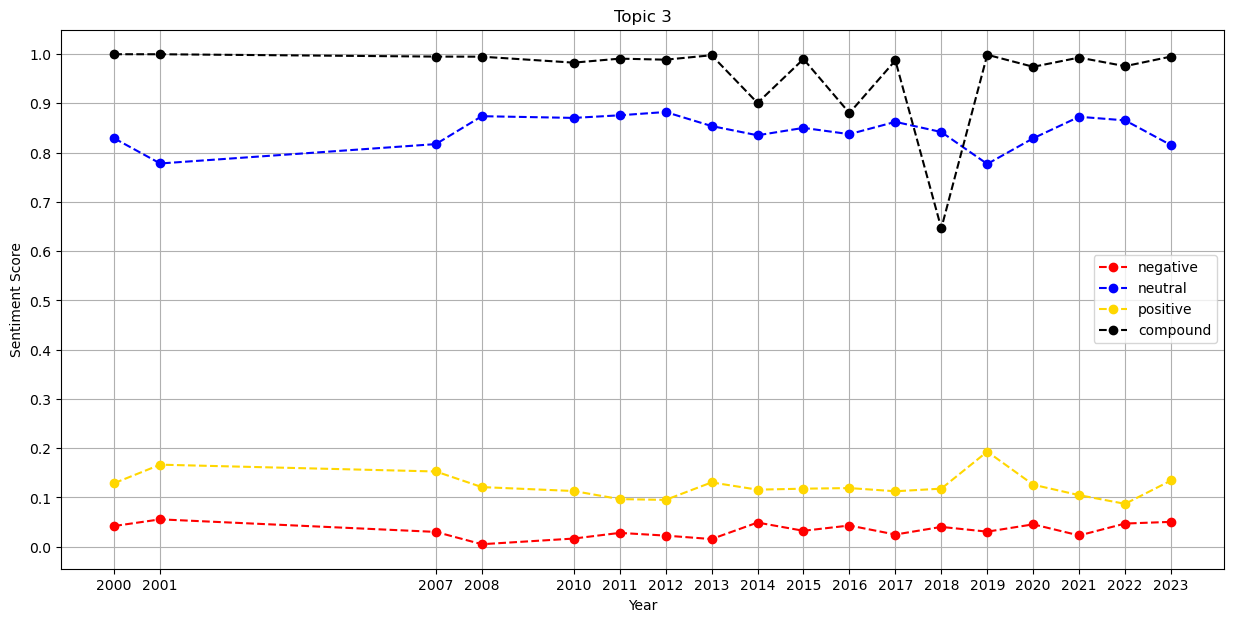
\includegraphics[width=\textwidth]{figures/sentiments/topic-3.png}
    \caption{\emph{autonomous, cyber, chatbots, ...}}
    \label{fig:sentiments-topic-3}
  \end{subfigure}
  \hfill
  \begin{subfigure}[b]{0.45\textwidth}
    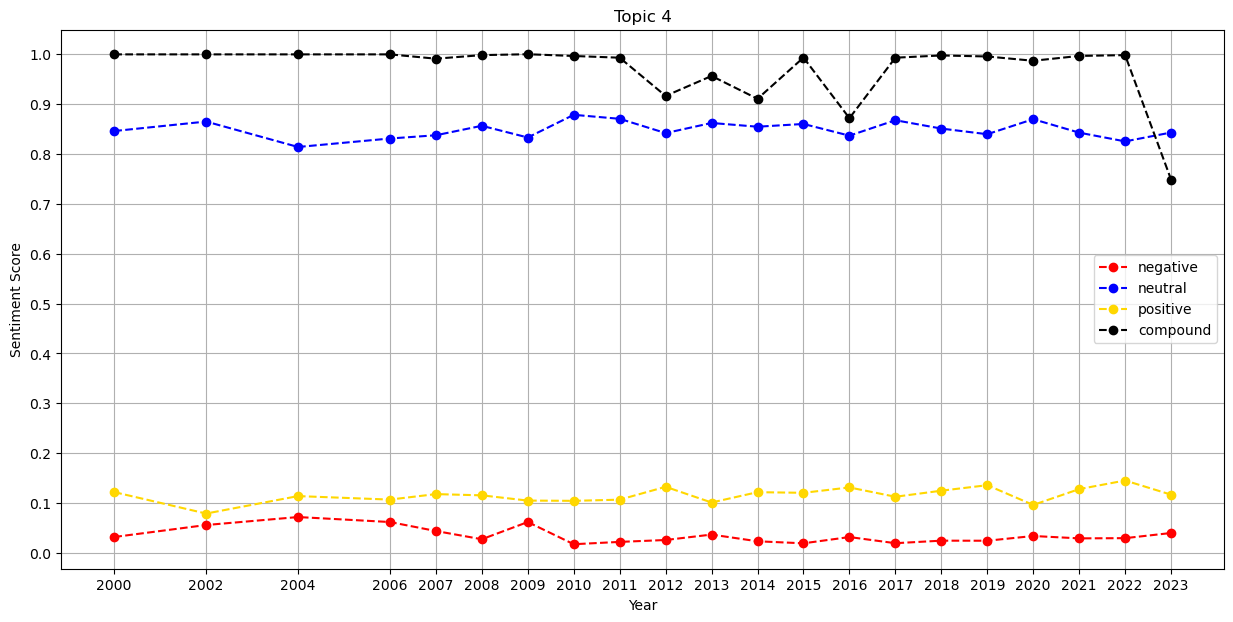
\includegraphics[width=\textwidth]{figures/sentiments/topic-4.png}
    \caption{\emph{mobile, app, enterprise, platform, ...}}
    \label{fig:sentiments-topic-4}
  \end{subfigure}

  \begin{subfigure}[b]{0.45\textwidth}
    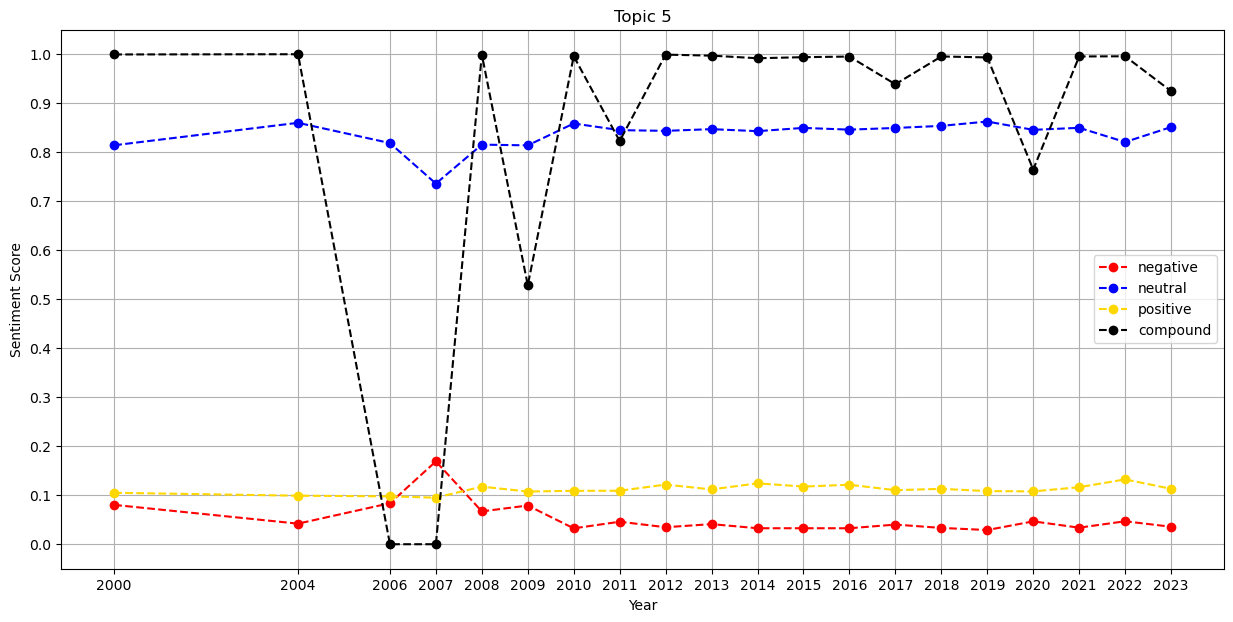
\includegraphics[width=\textwidth]{figures/sentiments/topic-5.png}
    \caption{\emph{ai, microsoft, human, future, microsoft, apple, ...}}
    \label{fig:sentiments-topic-5}
  \end{subfigure}
  \hfill
  \begin{subfigure}[b]{0.45\textwidth}
    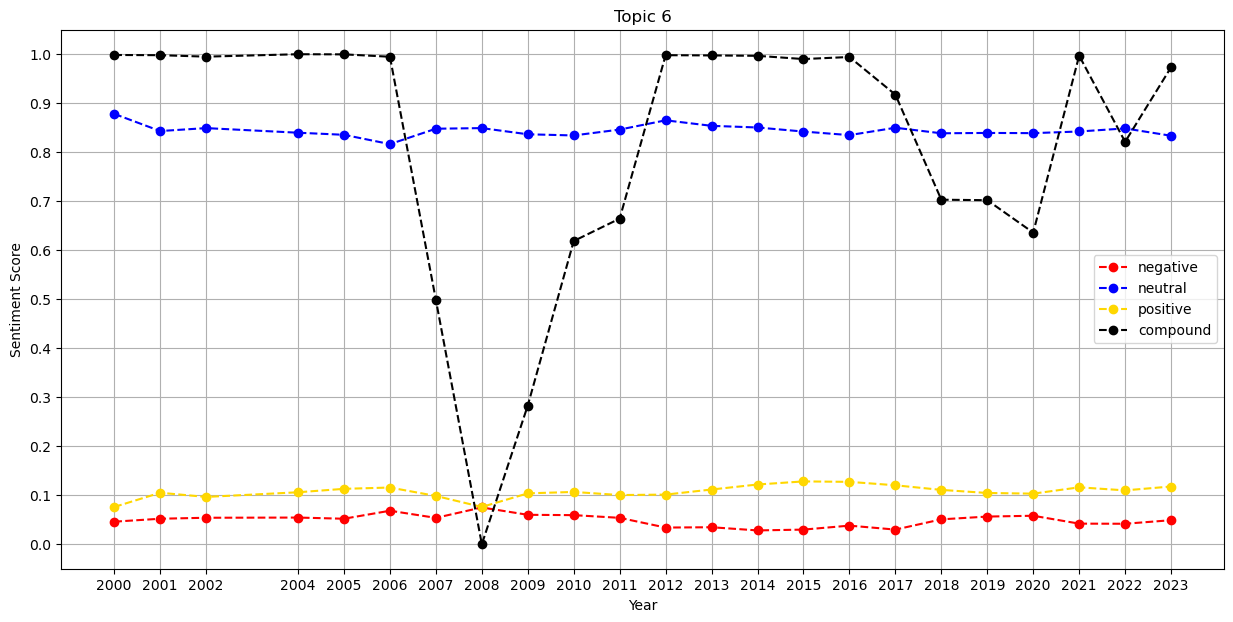
\includegraphics[width=\textwidth]{figures/sentiments/topic-6.png}
    \caption{\emph{deep, learning, deepmind, mit, google, ...}}
    \label{fig:sentiments-topic-6}
  \end{subfigure}
  \vskip\baselineskip
  \begin{subfigure}[b]{0.45\textwidth}
    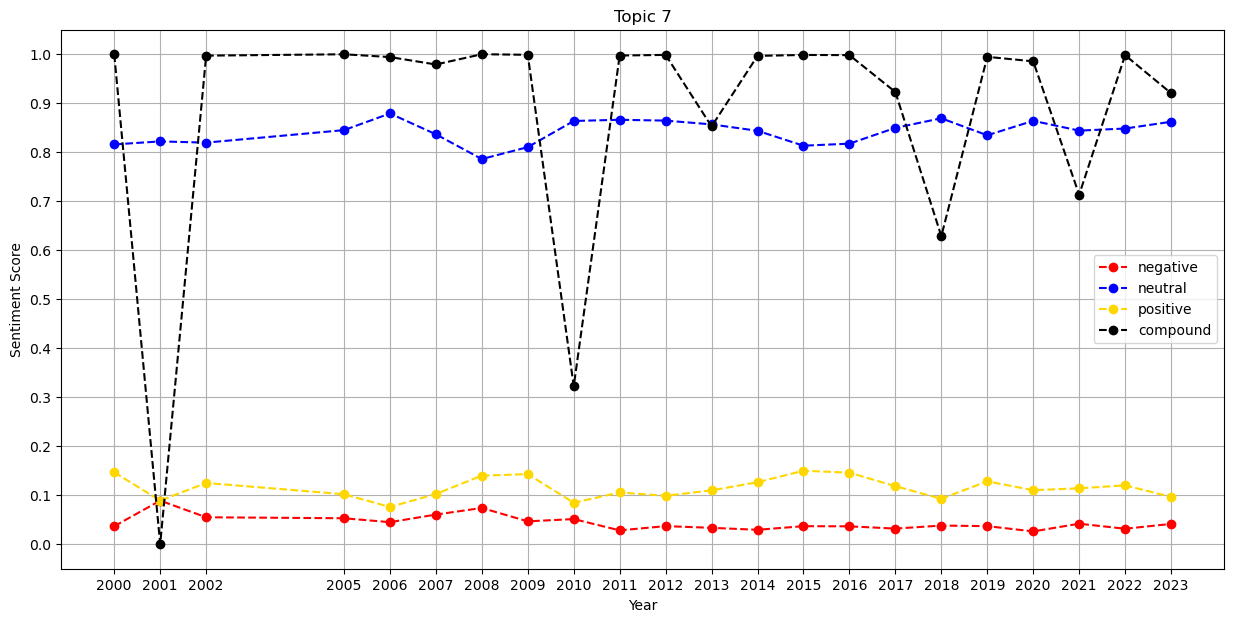
\includegraphics[width=\textwidth]{figures/sentiments/topic-7.png}
    \caption{\emph{cloud, windows, optimization, ...}}
    \label{fig:sentiments-topic-7}
  \end{subfigure}
  \hfill
  \begin{subfigure}[b]{0.45\textwidth}
    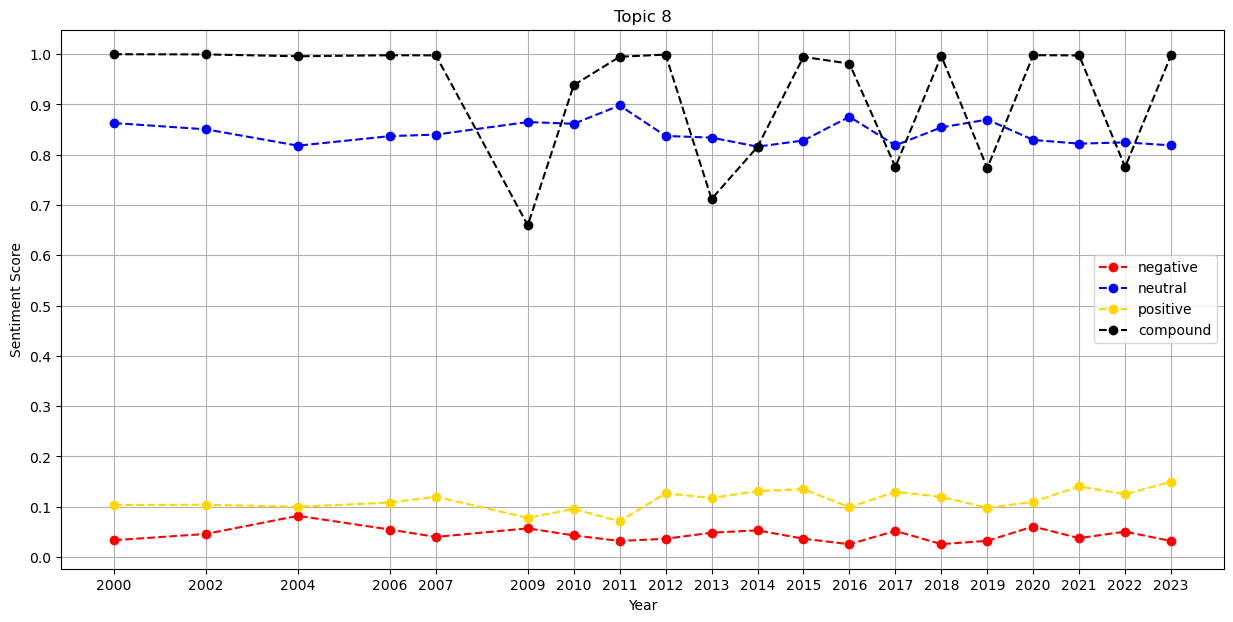
\includegraphics[width=\textwidth]{figures/sentiments/topic-8.png}
    \caption{\emph{metaverse, game, brain, world, covid, ...}}
    \label{fig:sentiments-topic-8}
  \end{subfigure}

  \begin{subfigure}[b]{0.45\textwidth}
    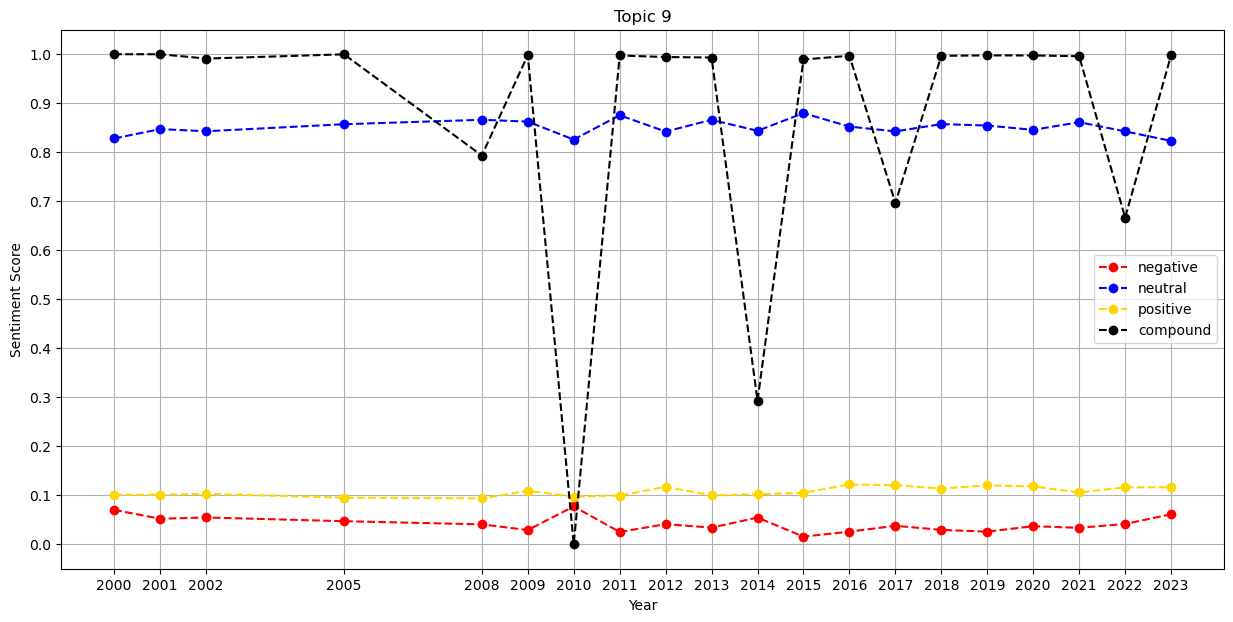
\includegraphics[width=\textwidth]{figures/sentiments/topic-9.png}
    \caption{\emph{developers, web, google, codex, raises, ...}}
    \label{fig:sentiments-topic-9}
  \end{subfigure}
  \hfill
  \begin{subfigure}[b]{0.45\textwidth}
    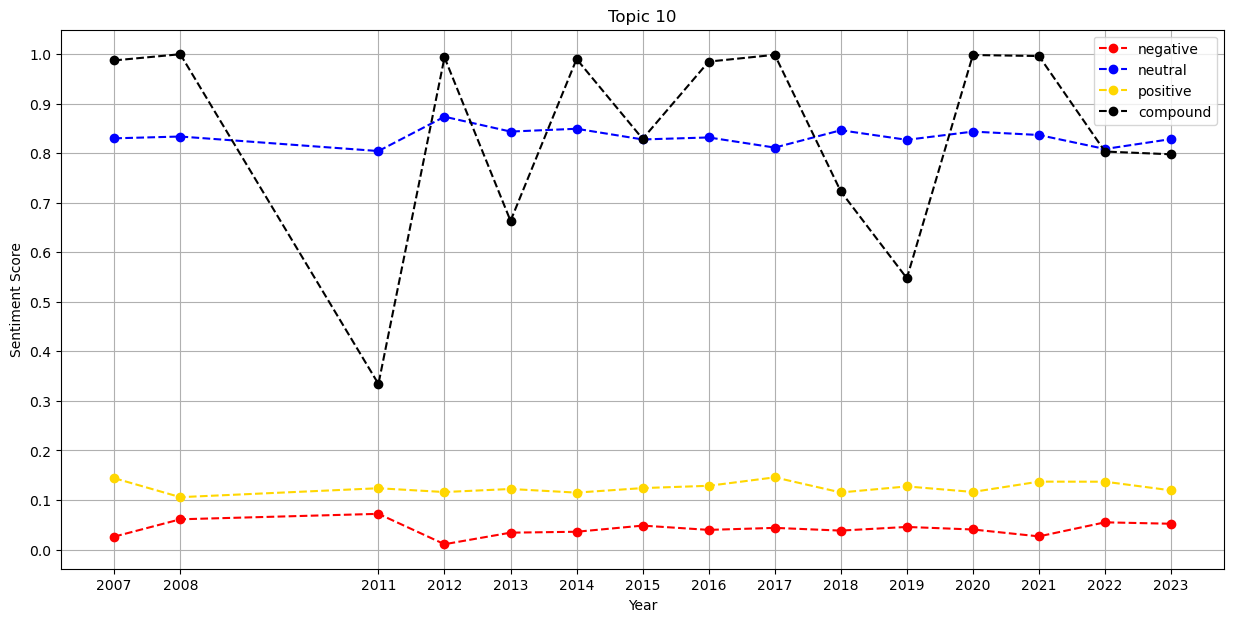
\includegraphics[width=\textwidth]{figures/sentiments/topic-10.png}
    \caption{\emph{security, software, real, health, ...}}
    \label{fig:sentiments-topic-10}
  \end{subfigure}
  \caption{Sentiment shifts across the top $10$ topics from $2000$ to $2023$.}
  \label{fig:sentiments-topics}
\end{figure}

The composite sentiment score for multiple of the top topics show
significant dips to (occassionally) zero in the periods between
$2005$ and $2011$. We believe this might be a result of
certain concepts prominent in the top topics not being
as prevalent in the news articles during that period.
For example, \cref{sub@fig:sentiments-topic-6} has \emph{deep, learning, deepmind, mit},
and \emph{google}
among its top words, but the \emph{deepmind} research lab was established
in $2010$~\cite{deepmind-about}. It is perhaps more interesting to look at
why the topic has high sentiment scores some earlier years ($2000$--$2004$),
but we leave that for future work.
